\documentclass[12pt,a4paper]{article}
\usepackage[utf8]{inputenc}
\usepackage{amsmath}
\usepackage{amsfonts}
\usepackage{amssymb}
\usepackage{graphicx}
\author{Group 3}
\title{Mini project Design Documentation}

\begin{document}

\begin{titlepage}
\begin{center}

\huge Software Requirements Specification\\[0.15cm]
\huge Squirrel Marking System\\[0.15cm]
\large \texttt{Version: 1.0}\\[1cm]

Organization:\\
\texttt{University of Pretoria: Group 3}\\[0.5cm]
GitHub:\\[0.01cm]
\begin{verbatim}
      https://github.com/Roach-301/CS301_Group3
\end{verbatim}

Authors:\\
\texttt{Johan Esterhuyse (10043283)\\
        Tokologo Machaba (12078027)\\
        Heelin Mistry (10299344)\\
        Pieter le Roux (1045486)\\
        Rudiger Roach (11004322)\\
        Thulasizwe Mavuso (29236259)}\\[1cm]
        
March 13, 2014
\end{center}
\end{titlepage}
\tableofcontents
\pagebreak
\section{Software architecture design}
\subsection{Choices of technologies}

The existing web server runs on Apache, therefore our system will continue the use thereof.\\\\
Django web server, running on Apache, will be our interface to run on.\\\\
Djangos Object Relational Mapper Will be used to persist information to the database.\\\\
Django unittest module will be used to perform unit tests with.
MySQL server allready runs on the CS server and this existing database will be used to pull information from and store information to.\\\\
The android application will be built using JAVA.

\subsection{Chosen frameworks}
Django application server will eventually be the framework onto which the system will be deployed and Djangos bundled Object-Relational mapper will be used to access the database.
\subsection{Chosen protocols}To send data between objects, it will first be encoded into JSON strings. JSON is an easy to use standard that can be parsed by most programming languages. This will enhance our ability to keep layers seperate from each other and just pass JSON strings between layers.
\subsection{Chosen libraries}
PDF creation will be done using iTextPDF from itextpdf.com. iTextPDF is open source with implementations on multiple different platforms. It is also licensed to enable re-use by developers.\\\\
PDF rendering will be done by using the PDFrenderer library from \\https://github.com/katjas/PDFrenderer. This library is LGPL-2.1 licensed and therefore fine for use by us. The library is written in JAVA and uses JAVA2D to render PDF documents.\\\\
To marshall and de-marshall JSON, Apache camel will be used from \\http://camel.apache.org/. This library is fully compatible with java and independent from the transport used.

\section{Application design}
\subsection{Back-end}
API:\\\\
\includegraphics[scale=0.5]{"BackEndAPI".jpg}
\pagebreak \\
Class Diagram:\\\\
\includegraphics[scale=0.4]{"BackEndClassDiagrams".jpg}

\subsection{Web Application}
\begin{itemize}
\item When the user directs to the system through one of the widely used browsers, a login screen is displayed. 
\item The login screen will be developed with HTML 5 and CSS3
\item It will consist of textboxes for the username and password and a button to send the information to the server.
\end{itemize}
\pagebreak
\textbf{Authentication Level}\\\\
LDAP Authentication:
\begin{itemize}
\item The system accesses the CS LDAP to validate and grant privilege to the logged in user.
\item When the user has been authenticated, pages are sent over to client browser over HTTPS \\
\end{itemize}
 \textbf{Home Page Level}\\\\
Possible actions according to privilege:
\begin{itemize}
\item A student will be directed to a page where he/she will only be able to view leaf and aggregate marks.
\item Markers will be presented with options to either:
\begin{itemize}
\item Create an assessment 
\item Edit marks for a specific student through a search interface
\item Delete marks and a text-area for the reason for doing so.
\item Changes committed will be displayed immediately through the use of JavaScript and JSON. 
\end{itemize}
\item Lectures will be able to:
\begin{itemize}
\item Manage information about the course through an easy to use interface that will make use of JSON to send data back and forth. 
\item Manage assessments:
\begin{itemize}
\item The lecturer will determine how marks are aggregated.
\item Lecture will decide which assessments are the leaf assessments.
\item He will specify how much each leaf assessment contributes to the aggregated mark.
\end{itemize}
\item Generate report
\begin{itemize}
\item The report can be generated into either a PDF or CSV at any level of granularity.
\end{itemize}
\end{itemize}
\end{itemize}
\section{Application layer Level}
\subsection{Protocols to be used}
\begin{itemize}
\item SOAP interface will be used through XML unmarshalling when accessed by other systems.
\item The application will run over, thus SOAP will run over HTTPS for a secure connection.
\end{itemize}
\subsection{Android Application}
The specifications of lower levels of granularity. 
Users will also have to be able to login to the application using their CS details. Users that should be able to use the application are markers, lecturers and students (who have android smart phones).\\

Students: 
\begin{enumerate}
\item  Students should be able to check their marks with the android application. 
\end{enumerate}



Markers: 

\begin{enumerate}
\item  After logging in markers will be able to insert the marks of students that have been assigned to them, for the subject they are marking. They should only be able to insert marks during the practical session (unless otherwise stated). 

\item  Markers can edit student marks but only for a reasonable circumstance. 

\item  Markers can search for students by student number, name and surname.

\item  Marks will be saved locally between updates to the server, so if anything happens to the application or the phone information will be saved, therefore no need to reinsert data already done
\end{enumerate}

 

Lecturers: 

\begin{enumerate}
\item  Lecturers should be able to login and choose between a menu of creating a session or viewing marks.

\item  When creating a session, a day, time and duration of the session should be assigned

\item  When assigning students and markers to session, they can be searched for by using student numbers, names and surnames. Multiple students can be assigned to a session by marking the students with a radio button.

\item  After assigning students and markers information should be saved locally between updates to the server.
\end{enumerate}

 

 The application:

\begin{enumerate}
\item  The system should log out after no more than 10 minutes of not being used. 

\item  The mobile uses MySQL database which it interacts with via the server. 

\item  Updates between the application and the server should be saved locally on the mobile memory.

\item  When a mark is sent to the system it should be checked to see if it was actually inserted, if not it should try again, if repeated failures are encountered an exception should be thrown telling the user to either retry or try to upload the marks later. 

\item  Mark sheets should lock after the practical session has ended, so that no more marks can be inserted (unless otherwise stated). 
\end{enumerate}

\noindent \textbf{API Specifications}\\\\
In the Android application the markers will be handling the marks as shown below:\\\\
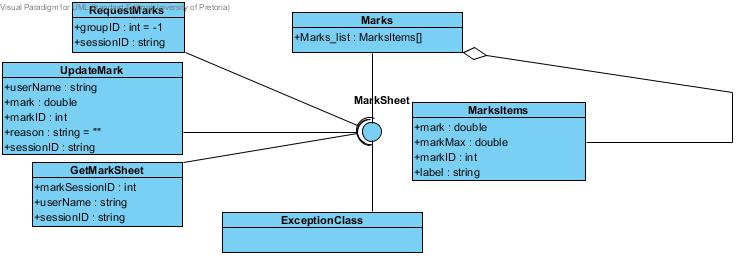
\includegraphics[scale=0.6]{APIMarks.jpg}\\\\
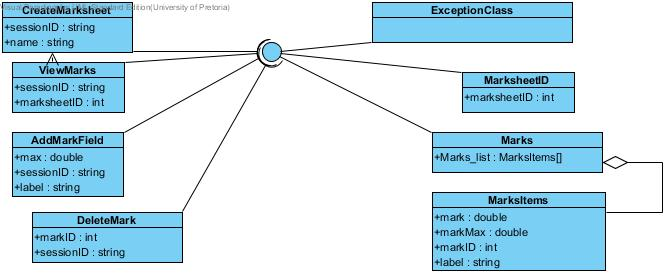
\includegraphics[scale=0.6]{APIMarksheet.jpg}\\

\noindent The android application will work according to sessions and whether or not they are open.\\\\
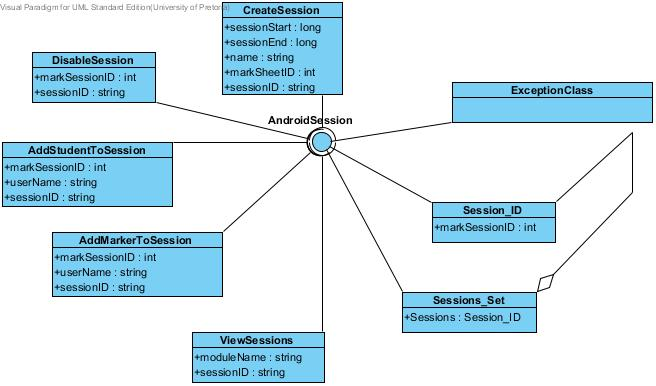
\includegraphics[scale=0.6]{APISession.jpg}\\\\

\pagebreak \noindent Class Diagrams
The Android Application will have the following structure:\\ 
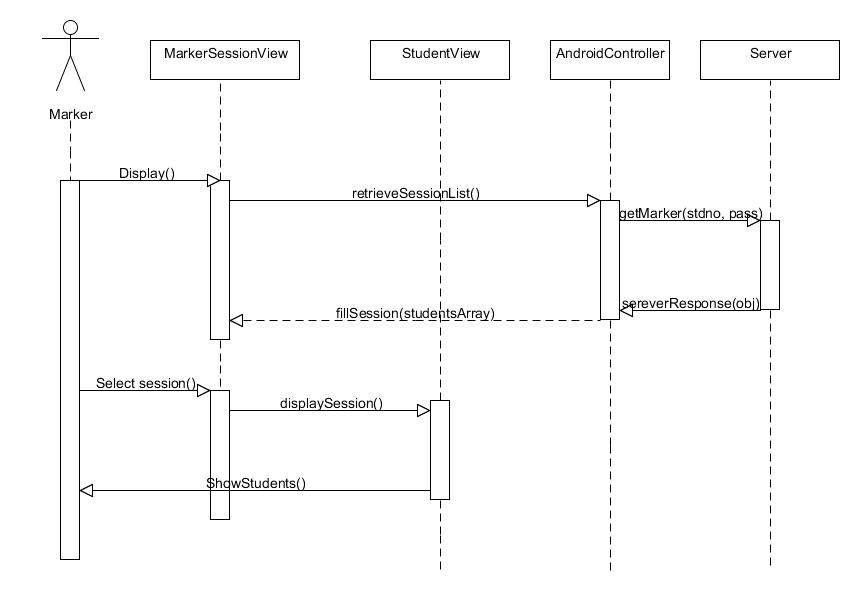
\includegraphics[scale=0.4]{androidSpecs.jpg}

\noindent Source:
\begin{verbatim}
http://developer.android.com/
\end{verbatim}

\noindent System Process Specifications\\
Login activity Diagram:


\textbf{User Interface Design:}


Login screen:\\
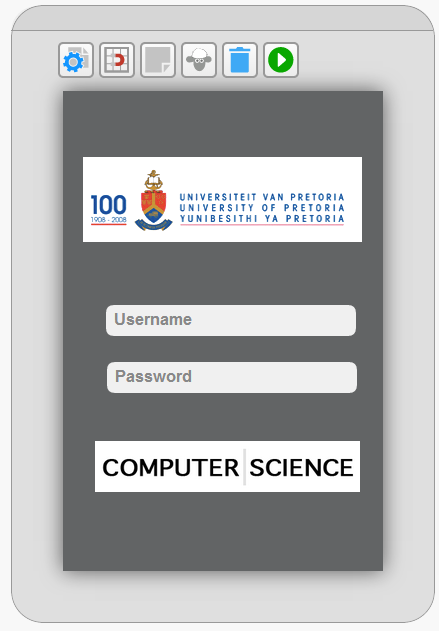
\includegraphics[scale=0.4]{login.png} \\
Students Menu:\\
\includegraphics*[scale=0.4]{login.png} 


\end{document}